\chapter{Process}

\section{Planning}

In the orientation report we proposed a planning where the workload was divided into different phases. We were able to keep up with this planning.
\\\\
The first step was to create an environment in which to develop and test the application. This meant gaining root access to a Samsung television and cross compiling the necessary libraries for it. This was achieved before the project had officially started which allowed us to begin development immediately.
\\\\
Our application heavily depends on libswift so the first goal was to be able to call libswift and use the library to stream and download files. This was achieved fairly quickly which meant we could start developing the fully functioning application. At the same time we also started development of the GUI in JavaScript. The main issue was creating the link between JavaScript and C++. Once we had settled for HTTP requests the development of the GUI and C++ side could be done in parallel although in the beginning the focus was on creating a command line controlled C++ application.
\\\\
As soon as there was a basic C++ application we also began writing tests using gtest. This made further development easier and bug tracking faster. Once the C++ part of the application was as good as finished, the last phase was to implement search functionality which required Python to be run on the television in order to run dispersy and DHT. Getting Python, including all the required modules, working on the television did not take long. Soon after that we were able to use dispersy and DHT to return search results.
\\\\
Once that all elements had been completed it was a matter of connecting them to create a fully functioning application. In the table below there is a more detailed week by week description of when what was done.
\\\\

\begin{table}
\centering
	\begin{tabular}[| l | l | l |}
		
		\hline
		Week & Date & Tasks completed \\
		\hline
		\hline
		1 & 30-04-2012 & 	\begin{itemize}
								\item 
							\end{itemize} \\
		\hline
		2 & 07-05-2012 &		\begin{itemize}
								\item 
							\end{itemize} \\
		\hline
		3 & 14-05-2012 &		\begin{itemize}
								\item 
							\end{itemize} \\
		\hline
		4 & 21-05-2012 &		\begin{itemize}
								\item 
							\end{itemize} \\
		\hline
		5 & 28-05-2012 &		\begin{itemize}
								\item 
							\end{itemize} \\
		\hline
		6 & 04-06-2012 &		\begin{itemize}
								\item 
							\end{itemize} \\
		\hline
		7 & 11-06-2012 &		\begin{itemize}
								\item 
							\end{itemize} \\
		\hline
		8 & 18-06-2012 &		\begin{itemize}
								\item 
							\end{itemize} \\
		\hline
		9 & 25-06-2012 &		\begin{itemize}
								\item 
							\end{itemize} \\
		\hline
		10 & 02-07-2012 &	\begin{itemize}
								\item 
							\end{itemize} \\
		\hline

\end{tabular}
\caption{Order of events}
\label{tab:planning}
\end{table}


\section{Testing}

We only wrote tests for C++ as this was the core of our application. We made use of the google test library which allowed for easy implementation of unit tests. The tests were developed in parallel with the development of the application which allowed for constant checking for bugs with every change. This way most bugs were immediately discovered and removed as soon as they appeared. Writing the tests also helped making the system robust and able to handle unexpected input and calls without crashing.
\\\\
Every class has its own test class and almost every method has its own tests, usually a trivial test and additionally a couple of tests with unexpected input or unexpected situations. Certain classes, especially DownloadManager, required test cases to call multiple different methods in order to test certain situations. Although this resulted in some relatively long test cases it did guarantee a solid application capable of handling a large range of exceptional situations.
\\\\
We chose not to fully test SearchEngine, the reason being that SearchEngine relies on dispersy and DHT. Both of these services are unreliable when it comes to returning search results, you do not always get the same results and sometimes you get no results. The testing environment requires a fixed return value every time. In order to achieve this we created a mock of the SearchEngine class which has the same functionality as the real SearchEngine except when it comes to searching. The mock always returns the exact same results which are hard coded in the mock. This allowed us to test HttpServer without having to worry about dispersy and DHT returning different values every time.

\section{Problems encountered}
This section focusses on all the important problems we encountered while developing the application for the TV. A brief explanation will be given per problem together with the solution we came up with.

\subsection{Rooting the television}
The first hurdle before we could even start developing was gaining root access to the television. We needed this to be able to install libraries and execute code. Rooting the television should not have been an issue as there are tutorials and an app that roots the television for you from SamyGO\cite{SamyGO}. The problem we ran into is that the televisions we got had a new firmware for which there was no way to root yet.
\\\\
We had a quick look into finding a vulnerability in the new firmware that would allow us to execute arbitrary code and gain root access. We did find a possible vulnerability in ffmpeg, in the part used to decode Matroska video files, but developing an exploit for this would have taken too long as we did not have any experience in this field.
\\\\
Another option was to downgrade the firmware to a previous version that would allow us to use the SamyGO app to gain root access. Samsung has not made the option of downgrading available, it is only possible to upgrade, so we had to trick the TV into thinking it was upgrading while actually it was installing old firmware. It is possible to install new firmware via a USB device which is what we initially tried. We took some old firmware, unpacked it, changed the version numbers inside, repacked it and recalculated the MD5 hash and changed that too so that they would match. Sadly, this is when we found out that the firmware also required a signature from Samsung which is something we did not have. This made downgrading via a USB device impossible.
\\\\
We contacted SamyGO to ask whether there was any way to downgrade to an older firmware. Initially the answer was no but after some prodding they allowed us to make use of a server they had set up which pretends to be the Samsung firmware update server. Apparently the online firmware update did not require a Samsung signature or they had access to it. Either way, we now had a television with an old firmware which allowed us to run the SamyGO app and root the TV.

\subsection{Installing missing dependencies}
Even though the SmartTV runs a linux kernel, not everything was available from the start, so we had to install a great number of packages on the TV.
For this purpose, we used cross-compiling toolchains to build executables compatible with the ARM \cite{arm} processors which resides in the TV. However, we failed
to fully compile some of these packages, of which the Python interpreter is one of the most important. The Python interpreter was needed because the dispersy and DHT modules 
developed by the Tribler team were written in Python. Since we had to use these modules in our application, we also needed to install Python on the TV. 
\\\\
We succeeded in cross-compiling and running the interpreter on the TV, but not in cross-compiling the standard Python-modules we need to run simple Python executables.
Our solution was to emulate the ARMv7 processor with QEMU \cite{qemu}. Within this emulation, we installed a copy of Ubuntu, \cite{ubuntu} in which we were able to install the Python package with the apt tool.
To achieve this, it was also needed to enable networking within QEMU. \cite{qemu-network} Then we copied the binary files to the TV, after which we could succesfully run the Python interpreter together with all its dependencies.
\\\\
Aside from Python, we also installed other applications via QEMU such as bash, sshd etc. to make it easier to work on the TV to accelerate the development.

\subsection{TCP RST packages}
It appeared that the Samsung TV sent TCP RST packages to itself after each HTTP request. TCP RST packages can be distinguished by looking at the fourth flag in the TCP header. This flag is the reset flag, which was activated in our case (see figure \ref{fig:TCP_RST}). Because of this, TCP connections to swift were interrupted each time a RST package was received, because the TCP connection was reset. This was a problem for file streaming, because the connection used by libswift to download the stream was continually interrupted, so the stream could not be played correctly. 
\\\\
We solved this problem by cross-compiling iptables\cite{iptables} for the TV, so we could set up some rules to block TCP RST packages. This required us to insert several kernel modules. Because this needs to be done each time the TV reboots, we added some rules to the init script of the TV so that these kernel modules are loaded automatically, together with the rules written for iptables (see \hyperref[sec:vusb_init]{appendix}).

\begin{center}
\begin{figure}[h]
	\centering
	\mbox{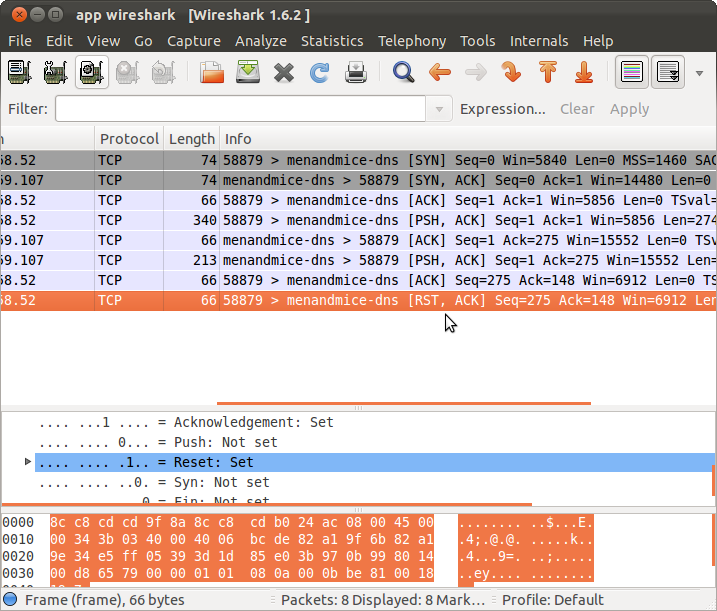
\includegraphics[width=1.2\textwidth]{Images/tcp_rst.png}}
	\label{fig:TCP_RST}
	\caption{Screenshot of wireshark. The RST package is highlighted in orange. Also, in the lower part of the screen it can be seen that the RST flag is set.}
\end{figure}
\end{center}

\subsection{Fork() and thread problem}
For testing purposes, we used a webserver written in C++ we found on the Internet. We were 
not aware, however, that this webserver was implemented so that it would call the fork() 
method each time a HTTP request was received. We were using p\_threads\cite{thread} to start several libevent\cite{libevent} loops needed for downloading files and p\_threads cannot access data directly within other processes. So we got the problem that the threads were not able to access the correct data.
\\\\
The problem was that fork() creates a new process, which is an exact copy of the parent 
process (See figure \ref{fig:fork_thread}). So all global variables and threads running 
within the process were also copied. Now, each time we tried to access a global variable, we 
noticed that the values of the variables were inconsistent because we were setting and 
reading the wrong variables. Unconsciously, we would set the value of a global variable, but 
read out the value of its copy instead, which has not been set yet. This caused unexpected 
behaviour of our application, on which we spent a lot of time. Strangely enough, this problem 
did not occur when we compiled and ran the program for our own pc\textquotesingle s, but only when we tried it on the TV.
\\\\
A solution is to implement pipes, which provide inter-process communication. With this, threads are able to access data outside their own process scope so the correct variables can be read. 
\\\\
In the end, we solved this problem by implementing a new HTTP server by ourselves, which makes use of the libevent library. This version of the webserver does not call the fork() method, so we did not have the problem of threads not being able to access the same data.

\begin{center}
\begin{figure}[h]
	\centering
	\mbox{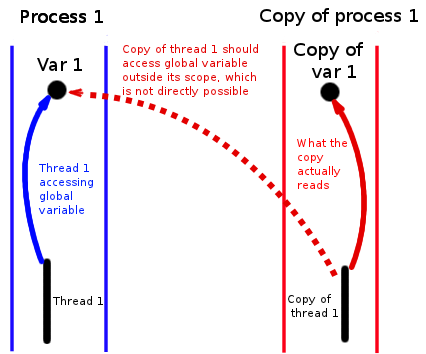
\includegraphics[width=0.8\textwidth]{Images/fork-thread.png}}
	\label{fig:fork_thread}
	\caption{The fork()-thread problem. Threads are accessing the wrong data.}
\end{figure}
\end{center}

\subsection{Communication between JavaScript and C++}
One of the first issues we encountered was how to link javascript to C++ so that we could call C++ functions from within the GUI and get return values back. Initially we wanted to use a language binder like SquirrelFish or a javascript engine for C++ like google V8. However due to the restrictions set by Samsung you are forced to develop the javascript app using their SDK and it is impossible to add any additional tools. This left us with the standard javascript functionality and the Samsung API. As Samsung does not allow any development outside of javascript there was no support for calling C++ applications in their API either. The only remaining option was to use HTTP requests which is part of the standard functionality in javascript.
\\\\
This did require us to be running an HTTP server in C++ which needs to be running before the javascript app had even been started. Newer version of the firmware also support HTML5 and websockets. This would allow for better two way communication betweem javascript and C++ rather than javascript constantly polling the HTTP server when it needs updates. The downside of this newer firmware is that there is no known way to gain root access yet which is why we could not use it.

\subsection{Starting the HTTP server}

Sending HTTP requests was the only way to communicate between javascript and C++ but there was no way to start the HTTP server in C++ from javascript. We needed to start the HTTP server as soon as the television was switched on. In principle it would have been possible to run the HTTP server as a daemon on start-up but it was not possible to edit the Samsung init scripts. SamyGO, however, also uses init scripts when they root the television which we could edit. Now whenever you root the television using SamyGO you also automatically start running the HTTP server for our application. This does mean that running SamyGO is required to be able to use our application.

\subsection{USB write speed}
Initially we were planning to use a USB storage device to store downloads and streams. As it turned out, the write speed of the TV to the USB device was so slow that streaming was not possible when using it to store the data. Downloading to an external USB device was also so slow that it was not practical to do so. This left us with only the internal memory of the TV for downloads and streams which is a very limited amount. This caused large files to be impossible to stream as they would fill the memory and cause the TV to hang. The maximum file size that can be downloaded is also very low as a result of this.
